% !TEX root = ../my-thesis.tex
%
\chapter{Particle neighborhood and anisotropic kernels}
\label{sec:particleneighborhood}

\section{From isotropic to anisotropic}

We explained the smoothing kernels used in \textbf{Smoothed Particle Hydrodynamics \myref{sec:sph}} above and called them isotropic - which can be thought of as "spherical" or radially homogenous. This property is necessary for simulation but leads to the most prominent visual artifacts of visualizing particle-based surfaces: Flat surfaces no longer look flat but rather bumpy. It can be evidently seen that the underlying representation is made up of points or spheres. The authors compared their method to multiple others, illustrating the need for a way of hiding spherical artifacts (see Figure 8 of Wu et al. \cite{Wu:2022}). To combat this, researchers have begun to develop anisotropic techniques for the extraction of surfaces from point clouds as soon as 2001 (Dinh et al. \cite{Dinh:2001}).

Interestingly, the main idea has not changed over the last 20 years seeing that Wu et al. use a very similar technique as described in that 2001 paper:
For a given point in space, the configuration of the neighboring points is characterized with a principal component analysis to retrieve the main axes along which the particles are distributed. This information is used to stretch the surface in a way that better fits the particles' distribution. This has the effect of preserving sharp features like edges and corners as well as flat, homogenous areas.

In our case, "stretching the surface" means transforming the input vector to the kernel function with a linear transformation matrix $\textbf{G}$ consisting of rotation and non-uniform scaling (further information below in \textbf{Particle classification \myref{sec:particleclassification}}):
\[
W_{a} ( \textbf{r}, \textbf{G} ) :=
c \space \det (\textbf{G}) \space P ( | \textbf{G} \textbf{r} | )
\]
Comparing to the isotropic kernel function $W$, the authors substitute $\frac{1}{h^3}$ for the determinant of $\textbf{G}$ and apply the linear transformation to the input of $P$.
This kernel can be reduced to the isotropic kernel by setting $\textbf{G} := h^{-1} \textbf{I}$ where $\textbf{I}$ is the three-dimensional identity matrix.

\section{Neighborhood definition}

The neighborhood $N$ of a point $\textbf{r}$ is defined as the set of the indices of all particles that lie in a sphere with radius $R_N$ around that point:
$$N (\textbf{r}, R_N) := \{ i \in \{ 0,...,n-1 \} : | \textbf{r}_i - \textbf{r} | < R_N \}$$

\section{Neighborhood search}

The authors did not mention the algorithm they used to find neighboring particles. The de facto standard spatial acceleration structure for SPH-related algorithms is the hash grid. For this reason, we opted to incorporate this approach as well, leaning on the explanation by Koschier et al. \cite{Koschier:2019}. A hash grid divides space into equally sized cells. A cell index can then be computed for an arbitrary point $\textbf{r}$ by dividing by the cell size $c$ and rounding each entry down to the closest integer:
\[
\begin{pmatrix} i \\ j \\ k \end{pmatrix} :=
\lfloor c^{-1} \space \textbf{r} \rfloor =
\begin{pmatrix}
\lfloor c^{-1} \space x \rfloor \\
\lfloor c^{-1} \space y \rfloor \\
\lfloor c^{-1} \space z \rfloor \\
\end{pmatrix}
\]
The cell index can then be hashed using any function $hash: \mathbb{Z}^3 \rightarrow \mathbb{Z}$ to retrieve an index into a table storing some data associated with the cell. In this case, we store a list of indices of particles lying in the cell.

We use a library called \textit{CompactNSearch} developed by Dan Koschier \cite{CompactNSearch} which is also used by the \textit{SPlisHSPlasH} framework \cite{SplishSplash} we use for dataset generation. It uses the technique described above to accelerate neighborhood search in a point cloud for a given neighborhood radius which is equal to the cell size $c := R_N$. The hashing function is efficient, consisting only of simple prime number multiplications (using prime numbers $p_0,p_1,p_2$) and XOR operations ($\otimes$):
\[
hash(i,j,k) :=
p_0 i \otimes
p_1 j \otimes
p_2 k
\]
Koschier keeps their implementation straightforward by using the C++ standard library's \textit{std::unordered\_map} as a hash table, providing the custom hash function mentioned above.

Each value of the hash table holds an array of integers representing the indices of the particles contained in the cell.

So, when querying the neighbors of a point $\textbf{r}$, every particle in the $3 \times 3 \times 3$ neighborhood of that cell has to be tested for inclusion. This is because the cells' width is equal to the search radius. The test looks as follows:
\[ |\textbf{r}_i - \textbf{r}| < R_N \]
or more efficiently as calculating a root is slower than multiplication:
\[ (\textbf{r}_i - \textbf{r})^2 < R_N^2 \]
We use two separate search grids:
\begin{enumerate}
    \item one for density calculation - for which we set $R_N := h$ -
    \item and one for anisotropy calculation - for which we set $R_N := 2h$.
\end{enumerate}

The first one is used whenever we compute $\rho(\textbf{r})$. Using the kernel's property of having finite support - meaning $W(\textbf{r}) = 0$ for $|\textbf{r}| \geq h$ -, the summation does not have to iterate over all particles of the system. Instead, we perform a neighborhood search to greatly reduce the number of operations necessary to calculate the density.

The second search grid is used for characterizing the neighborhood of each particle $i$ to obtain a transformation $\textbf{G}_i$. It is used in the anisotropic kernel function when computing $\rho$.

A naive loop over all $n$ particles means the evaluation of $\rho$ has a lower bound of $\mathcal{O}(n)$. Because accessing the hash table is a constant-time operation, spatial hashing reduces the time complexity to approximately $\mathcal{O}(\overline{|N|})$ where $\overline{|N|}$ is the expected number of neighbors.

It is also important to consider how cells are ordered in memory. Modern hardware implements extensive caching capabilities that are essential for performant software. Programmers are advised to keep memory locations that are accessed together close to each other. Since for every neighborhood search, 27 cells have to be looked up, it is beneficial to store these 27 cells as close to each other as possible. Koschier therefore sorts the grid in a z-curve arrangement, allowing for spatial coherence when arranging a three-dimensional grid in a one-dimensional array (see Figure \myref{fig:z-curve} for a two-dimensional illustration).

\begin{figure}[htb]
    \centering
    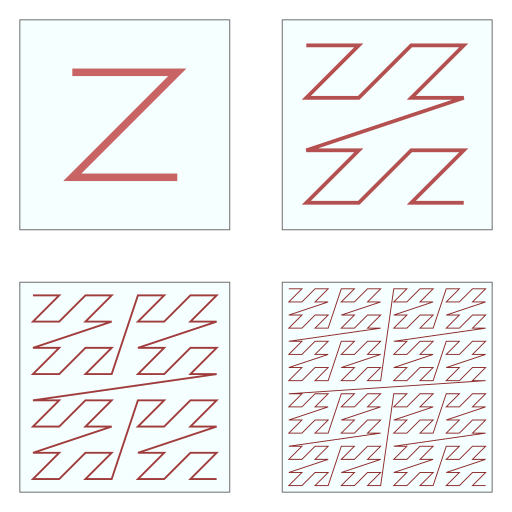
\includegraphics[width=0.75\textwidth]{my-gfx/figure-z-curve.png}
    \caption{A z-curve ordering of two-dimensional grids of varying sizes. The image comes from the public Wikimedia Commons repository \cite{ZCurve}.}
    \label{fig:z-curve}
\end{figure}


\section{Weighted Principal Component Analysis}

Principal component analysis is a common method of reducing the dimensionality of datasets to enable visualization in two or three dimensions (Koren et al. \cite{Koren:2003}). This is achieved by finding orthogonal axes that best fit the data and project it onto a subset of those axes. Since we are not dealing with high-dimensional data, we are not interested in reducing its complexity. Rather, we want to find the axes that most closely match the configuration of points in a small neighborhood. To do this, one has to compute the eigenvectors of the correlation matrix derived from the point set.

In this section, we explain the algorithm Wu et al. use to compute the principal components. It depends on the work of Yu and Turk \cite{Yu:2013} where an alteration of standard PCA is employed called Weighted Principal Component Analysis (WPCA). The key difference is that each point $\textbf{r}_j$ is assigned a weight $w_{j} \in \mathbb{R}$ that is used when computing the dataset's correlation matrix $\textbf{C}$ and mean $\overline{\textbf{r}}$.

We define the correlation matrix as not limited to evaluation at the particles' positions. This differs from our sources (Yu and Turk \cite{Yu:2013}) in that we can characterize the neighborhood around any point in space. The reason for this is explained below in \textbf{Implementation \myref{sec:particleneighborhood:implementation}}.
\[
\textbf{C}(\textbf{r}) :=
\frac{1}{\sum_j w_{j}}
\sum_j w_j (\textbf{r}_j - \overline{\textbf{r}}) (\textbf{r}_j - \overline{\textbf{r}})^T
\]

\[
\overline{\textbf{r}} :=
\frac{1}{\sum_j w_j}
\sum_j w_j \textbf{r}_j
\]
For weights, some isotropic smoothing kernel $W$ is used. We use the one described in \textbf{Smoothed Particle Hydrodynamics \myref{sec:sph}}:
\[ w_j := W(\textbf{r}_j - \textbf{r}) \]
Applying weights to the particles' positions can be interpreted as an analogy to the SPH method. It also reduces visual artifacts because there is no strict boundary between lying inside and outside the neighborhood of a point.

After computing $\textbf{C}$, an eigendecomposition is performed on this matrix. The matrix is decomposed into a rotation $\textbf{R}$ and a scaling $\bm{\Sigma}$ containing $\textbf{C}$'s eigenvalues on its diagonal (see equation 12 in Yu and Turk \cite{Yu:2013}):
\[ \textbf{C} = \textbf{R} \bm{\Sigma} \textbf{R}^T \]

\section{Singular neighborhood configurations}

Some neighborhood configurations might yield a correlation matrix whose determinant is close or equal to zero. This can happen when all points lie on the same plane. In this case, the eigendecomposition returns a small eigenvalue leading to exploding numbers when computing $\bm{\Sigma}^{-1}$. To address this problem, Yu and Turk introduce a minimum for each eigenvalue as a fraction of the largest one. This way, the deformation can be controlled and parameterized to fit different use-cases.

Assuming $\sigma_1 \geq \sigma_2 \geq \sigma_3$, a new $\tilde{\bm{\Sigma}}$ is constructed with the altered eigenvalues, limiting the ratio of two eigenvalues to a constant $k_r$ (see equation 15 in Yu and Turk \cite{Yu:2013}):
\[ \tilde{\sigma}_k := \max \{ \sigma_k, \frac{\sigma_1}{k_r} \} \]
\[
\tilde{\bm{\Sigma}} :=
\begin{cases}
k_s \text{diag}(\tilde{\sigma}_1, \tilde{\sigma}_2, \tilde{\sigma}_3) & |N| > N_{\epsilon}, \\
k_n \textbf{I} & else
\end{cases}
\]
\[ \tilde{\textbf{C}} := \textbf{R} \tilde{\bm{\Sigma}}^{-1} \textbf{R}^T \]

We define $\tilde{\textbf{C}}(\textbf{r})$ as a function that computes $\textbf{C}(\textbf{r})$ as above and alters it, returning $\tilde{\textbf{C}}$.

The parameters of this algorithm are explained briefly. Note that they are dataset-dependent and the provided values work well with our dataset.
\begin{enumerate}
    \item $k_r \geq 1$ limits the maximum deformation relative to the largest eigenvalue. Large values lead to large deformations. We used $k_r := 2$.
    \item $k_s$ merely scales all eigenvalues. We used $k_s:= 2000$.
    \item $N_{\epsilon}$ is a threshold for the number of neighbors $|N|$. The deformation is not applied for really small neighborhoods. In this case, particles are displayed as spheres whose radius can be adjusted with $k_n$. This will prevent spray particles with few neighbors to be displayed as big ellipsoids. We set $N_{\epsilon} := 15$ and $k_n := 1$.
\end{enumerate}

In the following, the altered covariance matrix $\tilde{\textbf{C}}$ will be used to retrieve a transformation from isotropic to anisotropic space.

\section{Particle classification}
\label{sec:particleclassification}

\begin{figure}[htb]
	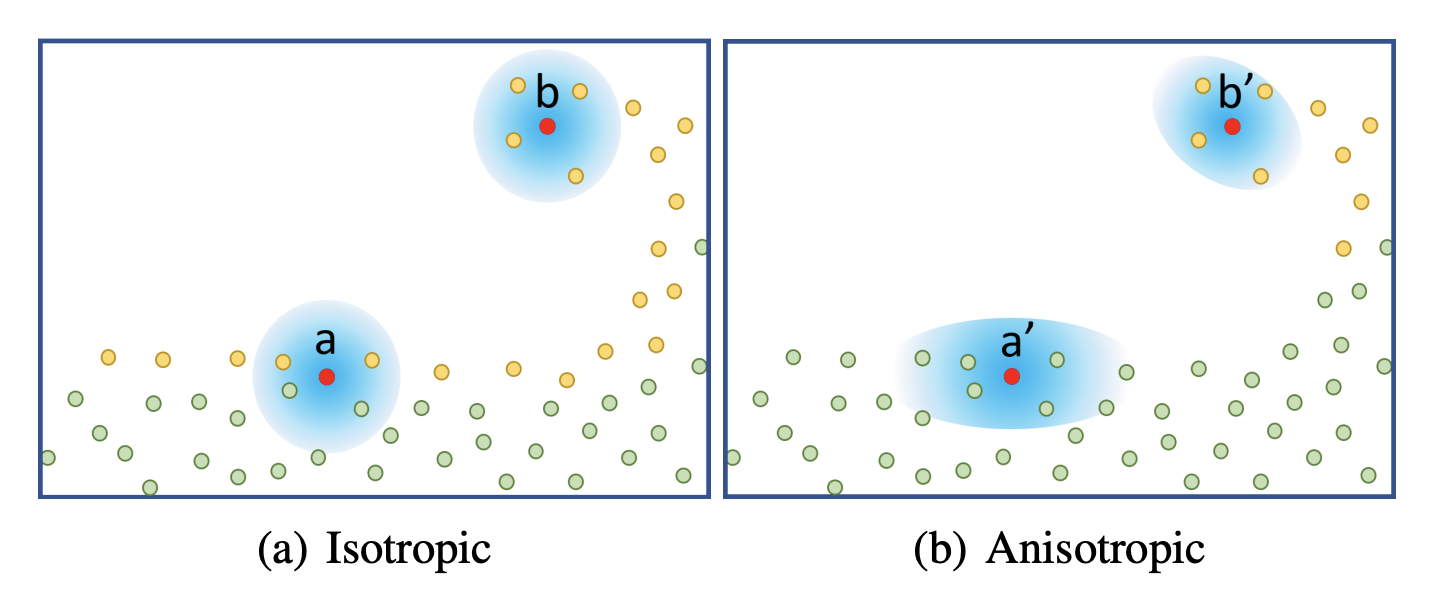
\includegraphics[width=\textwidth]{my-gfx/figure-anisotropic.png}
	\caption{This is figure 4 of the paper by Wu et al. \cite{Wu:2022}. It shows how anisotropic kernels help with correctly classifying particles located close to the surface of the fluid.}
	\label{fig:particleneighborhood:anisotropic}
\end{figure}

In order to reduce the number of ray marching steps near small bundles of particles, they have to be classified as either belonging to a dense fluid area ("aggregated") or to a sparse area (non-aggregated, splash particles). For this, the density is evaluated at each particle's position and compared to a constant. When using isotropic kernels for the density calculation, this will lead to misinterpretations at the surface of the fluid, even in aggregated locations (Figure \myref{fig:particleneighborhood:anisotropic}). Therefore, the authors suggest to characterize the particle's neighborhood as explained above and construct a transformation matrix $\textbf{G}_i$ for the particle to be used as an input to the anisotropic kernel $W_a$. $\textbf{G}_i$ is a transformation into the coordinate system represented by $\tilde{\textbf{C}}$, so it has to be the inverse of $\tilde{\textbf{C}}$ (note that $\textbf{R}$ is a rotation matrix, therefore $\textbf{R}^{-1} \equiv \textbf{R}^T$):
\[
\textbf{G}_i :=
h^{-1} \tilde{\textbf{C}}_i^{-1} =
h^{-1} (\textbf{R} \tilde{\bm{\Sigma}} \textbf{R}^T)^{-1} =
h^{-1} \textbf{R}^{-T} \tilde{\bm{\Sigma}}^{-1} \textbf{R}^{-1} =
h^{-1} \textbf{R} \tilde{\bm{\Sigma}}^{-1} \textbf{R}^T
\]
where $\tilde{\textbf{C}}_i := \tilde{\textbf{C}}(\textbf{r}_i)$ is the altered correlation matrix from above evaluated at the particle's position $\textbf{r}_i$.

Now, to compute the density at $\textbf{r}$, we use the anisotropic kernel function and only take those particles into consideration which are in the neighborhood $N$ of $\textbf{r}$:
\[
\rho(\textbf{r}) = m \sum_{i \in N(\textbf{r}, h)} W_a(\textbf{r}_i - \textbf{r}, \textbf{G}_i)
\]

This leads to a significant improvement in image quality as can be seen in Figure \myref{fig:anisotropy}.

\begin{figure*}
    \centering
    \begin{subfigure}[b]{0.475\textwidth}
        \centering
        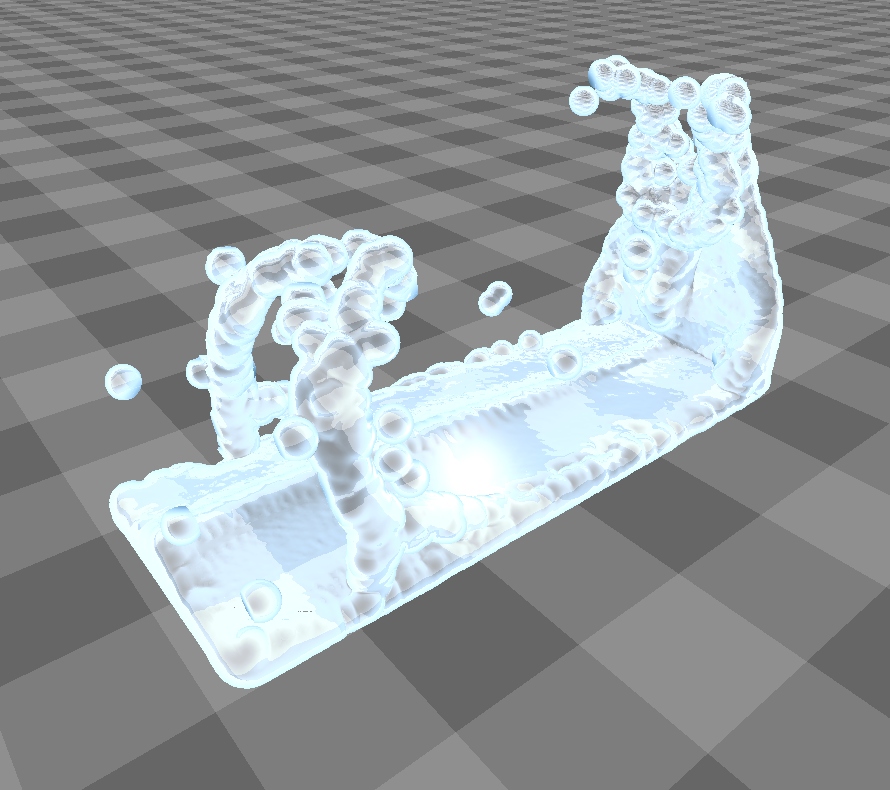
\includegraphics[width=\textwidth]{my-gfx/figure-anisotropy-1.png}  
    \end{subfigure}
    \hfill
    \begin{subfigure}[b]{0.475\textwidth}  
        \centering 
        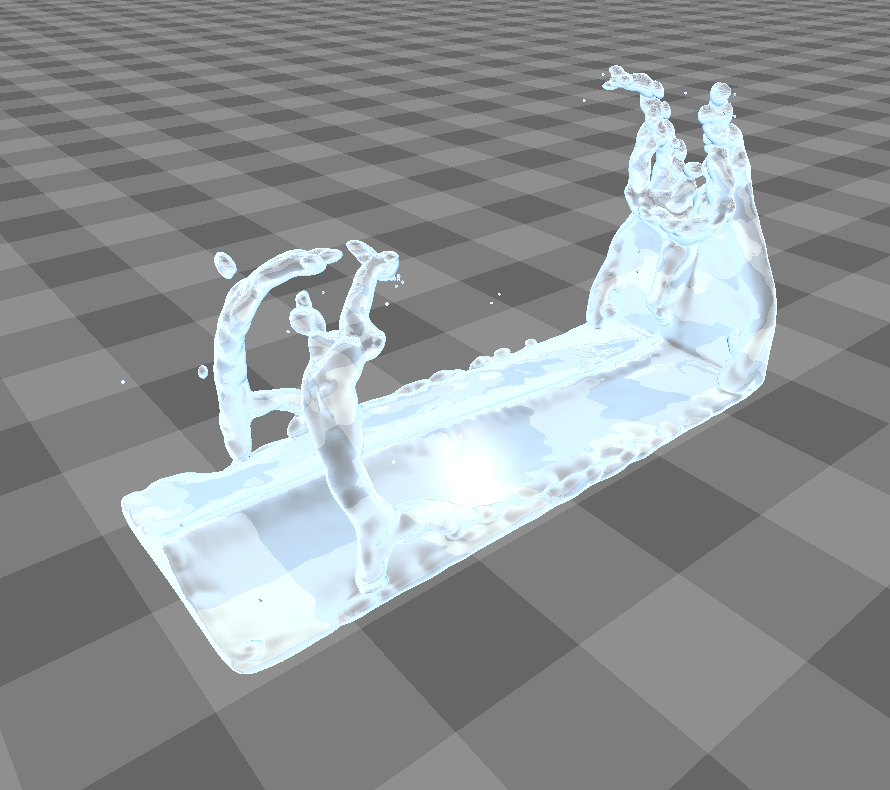
\includegraphics[width=\textwidth]{my-gfx/figure-anisotropy-2.png} 
    \end{subfigure}
    \vskip\baselineskip
    
    \caption{\textit{Left}: A visualization frame with isotropic kernels. Particles appear spherical and homogenous. \textit{Right}: The same scene with anisotropic kernels. The deformation is dependent on the neighborhood of each particle, creating a more interesting picture.}
    \label{fig:anisotropy}
\end{figure*}


\section{Implementation}
\label{sec:particleneighborhood:implementation}

Because the correlation matrix $\textbf{C}$ representing a neighborhood configuration is symmetric (see the following equation) and real and therefore self-adjoint - meaning $\textbf{C} = \overline{\textbf{C}^T}$ and specifically $\overline{\textbf{C}^T} = \textbf{C}^T$ for real matrices -, an algorithm called \mbox{\textit{SelfAdjointEigenSolver}} of the \textit{Eigen} library can be employed.
In the following equation, the brackets are used to differentiate indices from one another. We use $[\textbf{C}_i]_{mn}$ to refer to the element in the $m$-th row and $n$-th column of matrix $\textbf{C}_i$. Likewise, $[\textbf{x}_i]_n$ refers to the $n$-th entry of the vector $\textbf{x}_i$.
\[
\textbf{C}(\textbf{r}) :=
\frac{1}{\sum_j w_{j}}
\sum_j w_j (\textbf{r}_j - \overline{\textbf{r}}) (\textbf{r}_j - \overline{\textbf{r}})^T
\Rightarrow
\]
For $n,m = 1, 2, 3$:
\begin{align*}
[\textbf{C}(\textbf{r})]_{mn} &=
\frac{1}{\sum_j w_j} \sum_j w_j \space [\textbf{r}_j - \overline{\textbf{r}}]_m \space [\textbf{r}_j - \overline{\textbf{r}}]_n
\\ &=
\frac{1}{\sum_j w_j} \sum_j w_j \space [\textbf{r}_j - \overline{\textbf{r}}]_n \space [\textbf{r}_j - \overline{\textbf{r}}]_m
\\ &=
[\textbf{C}(\textbf{r})]_{nm}
,
\end{align*}

of which follows that $\textbf{C} = \textbf{C}^T$. This is also apparent because the outer product $\textbf{x} \textbf{x}^T$ itself is symmetric.

\textit{Eigen} uses a direct computation of eigenvalues and -vectors for three-by-three matrices by solving the equation $\textbf{A} \textbf{x} = \lambda \textbf{x}$ for the self-adjoint matrix $\textbf{A}$. There are iterative algorithms to achieve more accurate results but for the sake of performance, we chose to use the direct method.

Note that some math libraries automatically sort the computed eigenvectors by their associated eigenvalues in descending order. Others do not to reduce performance overhead when sorting is not needed. \textit{Eigen} belongs to the latter category. We could not rely on the eigenvalues being sorted, which was one source of errors during development.

\textbf{Note } At first, we performed the PCA at every step of the ray marching process. This led to greater visual fidelity as the granularity of the neighborhood determination was not restricted to the particle positions. But pre-computing the PCA for every particle up front - as Wu et. al suggest and as elaborated above - and using the resulting neighborhood matrix $\textbf{G}_i$ during ray marching is significantly faster while still bringing the advantages of anisotropic kernels. It could however be possible to perform the characterization during ray marching by fully porting the program to the GPU. Evaluations concerning this will have to be made in the future.

When finding the neighboring particles using the hash grid for neighborhood characterization, we use a search radius of twice the particles' radius: $R_N := 2h$. We found this to be a good compromise between over- and underfitting of the principal axes.

\section{Recap}

We have now introduced the transition from isotropic to anisotropic kernel functions and its necessity for high-quality surface reconstruction. We will now discuss the need for classification of particles into two groups. Furthermore, the key propositions of our primary source will be introduced and its effects will be evaluated.
